% Définition du nom du chapitre
\chapter[Deep convolutional neural networks to monitor coralligenous reefs: operationalizing biodiversity and ecological assessment]{Chapitre 1: Deep convolutional neural networks to monitor coralligenous reefs: operationalizing biodiversity and ecological assessment} \label{chapitre1-deep}

\pagestyle{main}

%%%%%%%%%%%%%%%%%%%%%%%%%%%%%
%%% Figure cover chapitre %%%
%%%%%%%%%%%%%%%%%%%%%%%%%%%%%
\begin{center}
\begin{tikzpicture}
  \def\ig{%
   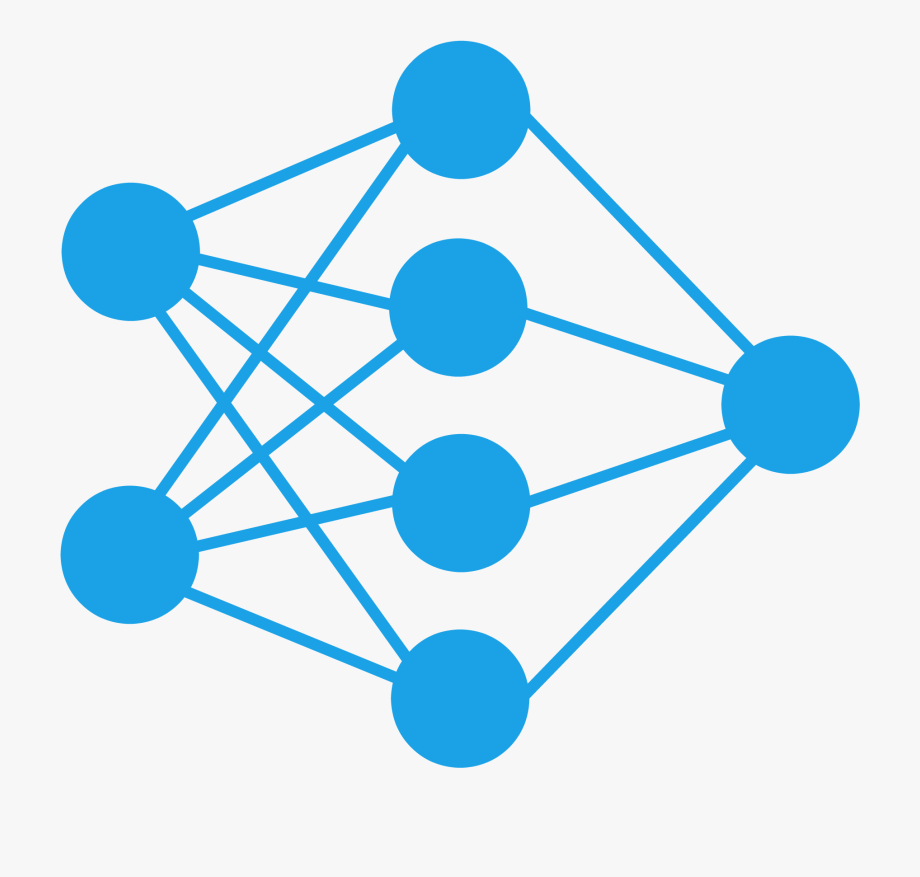
\includegraphics[width=0.5\linewidth,keepaspectratio]{./3_chapitre1/cover.png}}
 \node [inner sep=0pt](mypicture) at (0,0) {\phantom{\ig}};
 \clip[rounded corners=5mm] ($(mypicture.south west)+(\bord,\bord)$) rectangle ($(mypicture.north east)-(\bord,\bord)$);
 \node[inner sep=0pt](mypicture) at (0,0) {\ig};
\end{tikzpicture}
\end{center}

% Bullet points du début de chapitre
\begin{center}
\begin{colbox}{resume}
  \vspace{-2pt}
{\color{textresume}\small
\begin{itemize}[leftmargin=0in]\itemsep3pt
\item Nous avons entraîné un réseau de neurones convolutifs sur une base de données de près de \textbf{350 000} pour \textbf{61 classes} de coralligène et de substrat ~;
\item Le réseau final obtient une précision de \textbf{72.59 \%} sur 61 classes~;
\item La bonne calibration du réseau permet de faire une classification semi-automatique et de classer \textbf{67.48 \%} du jeu de données avec une précision de \textbf{85.65 \%}~;
\item En simplifiant la tâche de classification à 15 classes majeures, la précision atteint \textbf{84.47 \%}, soit une \underline{précision similaire à celle d'un expert taxonomiste}~;
\item Prédiction d'indicateurs de biodiversité et d'état de santé~:
\begin{itemize}
  \item Shannon~: bonne qualité prédictive (corrélation de Spearman 0.74)~;
  \item CAI~: qualité prédictive moyenne (corrélation de Spearman 0.61)~;
\end{itemize}
\end{itemize}
}
\vspace{-2pt}
%\end{fullminipage}
\end{colbox}
\end{center}

\clearpage

\noindent\textbf{Deep convolutional neural networks to monitor coralligenous reefs: operationalizing biodiversity and ecological assessment}

% Auteurs
\noindent Guilhem Marre, Florian Holon, Sandra Luque, Pierre Boissery et Julie Deter

% NB sans indentation
\noindent\textit{En cours de révision dans...}

\noindent\textbf{Abstract}


\noindent\textbf{Keywords}

% Introduction
\section{Introduction}\label{chapitre1_1}

\section{Related work}\label{chapitre1_2}

\section{Data}\label{chapitre1_3}

\section{Methodology}\label{chapitre1_4}

\section{Experimental settings}\label{chapitre1_5}

\section{Results}\label{chapitre1_6}

\section{Discussion}\label{chapitre1_7}

\section{Conclusions}\label{chapitre1_8}

\newpage